\subsection{Canales de decaimiento y tasas de ramificación}

Siguiendo a \cite{Cottingham.2001, Basdevant.2005, Krane.1987} los canales de desintegración (\textit{decaimiento}) son los posibles mecanismos en que una partícula puede fraccionarse, estos se muestran en la figura \ref{channels}.

\begin{figure*}%[H]
    \begin{center}
        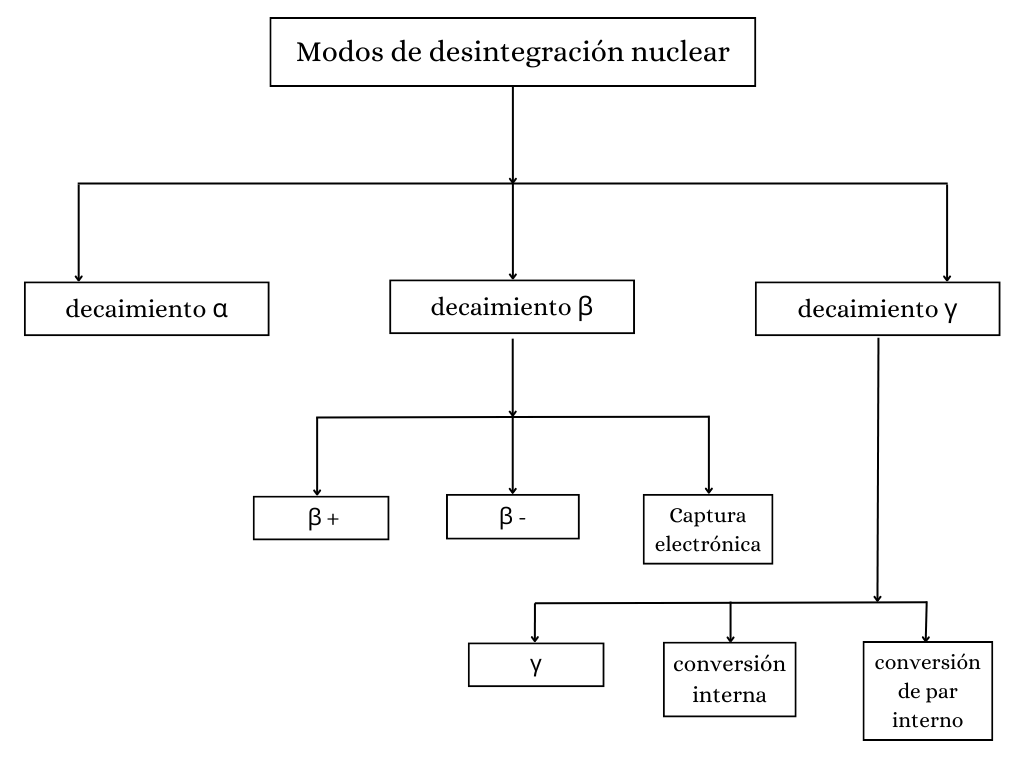
\includegraphics[scale=0.5]{imagenes/decay.png}
        \caption{Canales de desintegración para un radionúclido.}\label{channels}
    \end{center}
\end{figure*}

\noindent La desintegración radiactiva se produce a través de la emisión de diferentes tipos de radiaciones corpusculares, explica \cite{Krane.1987}. Los principales son: 

\begin{itemize}
	\item Radiación alfa ($\alpha $):  la partícula emitida corresponde a un núcleo de helio. La masa del nuevo núcleo disminuye en cuatro unidades, con relación al núcleo inicial. 
	
	\item Radiación beta ($\beta $): la partícula emitida es un electrón o un anti-electrón como consecuencia de la transmutación de un neutrón en protón, o al revés. El número atómico de masa permanece igual. Un neutrino  se lleva la energía complementaria liberada en la transformación. 
	
	\item Radiación gamma ($\gamma $): es un tipo de radiación electromagnética que transporta el exceso de energía de un núcleo inestable o metaestable. 
\end{itemize}

Los diversos modos de desintegración de un núcleo radiactivo son catalogados de acuerdo con la emisión del núcleo atómico:

\begin{itemize}
	\item Decaimiento Alfa:
	
	En este proceso, el núcleo padre se desintegra para dar un núcleo hijo y una partícula $\alpha$ ($^{4} He$). 
	
	\item Decaimiento Beta:
	
	En este proceso, el núcleo padre se desintegra para dar un núcleo hijo y una partícula $\beta $. La desintegración $\beta $ se subdivide en tres categorías, cuya descripción se sigue de la discusión desarrollada en \cite{Cottingham.2001, Krane.1987, Das.2009, Martin.2009}: 
	
    \begin{itemize}
    	\item \textbf{Emisión de electrones o $\beta^{-}$}: al desintegrarse el núcleo padre una partícula $\beta ^{-}$ y un anti-neutrino son expulsados. El número de masa del núcleo hijo es igual al del padre y el número atómico es mayor que el del padre por una unidad. 
    	
    	\item \textbf{Emisión de anti-electrones o $\beta^{+}$}: al decaer el núcleo padre una partícula $\beta^{+}$ y un neutrino son expulsados. El número de masa del núcleo hijo es el mismo que el del padre y el número atómico es una unidad menor que el del padre. 
    	
    	\item \textbf{Captura de electrones}: el núcleo padre captura uno de los electrones orbitales emitiendo un neutrino. El número de masa del núcleo hijo es igual al del padre, pero su número atómico disminuye en una unidad. 
 	\end{itemize}
 
	\item Decaimiento Gamma: las desintegraciones alfa y beta de un núcleo radiactivo pueden dejar al núcleo hijo en un estado excitado. Esta energía excedente puede puede perderse en forma de radiaciones electromagnéticas, llamadas rayos g. Dichos rayos pueden ser absorbidos por electrones orbitales y dar lugar a una creación de pares electrón-antielectrón.
\end{itemize}

\subsection{Leyes de la desintegración nuclear}

\noindent Siguiendo a \cite{Krane.1987}, las leyes de la desintegración radiactiva son: 
\begin{enumerate}
    \item Existe la misma probabilidad de que todos los núcleos de un elemento radiactivo se desintegran. 
 	
    \item La tasa de desintegración espontánea de un elemento radiactivo es proporcional al número de núcleos presentes en ese momento.
 	
\end{enumerate}

\noindent Matemáticamente, y en concordancia con \cite{Podgorsak.2016}, se puede escribir un modelo para la ley de desintegración radiactiva como: 

\begin{equation*}
    \dv{N}{t} \propto N
\end{equation*}

\noindent donde $N$ es el número de átomos presentes en el tiempo $t$. Eliminando el signo de proporcionalidad, obtenemos: 

\begin{equation}
\dv{N}{t} = -\lambda N\label{ecuaciondiferencialN}
\end{equation} 

\noindent Donde $\lambda $ se conoce como constante de decaimiento del elemento. El signo negativo indica que a medida que el tiempo $t$ aumenta, el número de núcleos $N$ disminuye. La ecuación \ref{ecuaciondiferencialN} puede resolverse mediante variable separable, notando que

\begin{equation}
\frac{\dd{N}}{N} = -\lambda \dd{t},
\end{equation} 

\noindent de integrar esto se obtiene: 

\begin{equation}
\ln( \lambda ) = -\lambda t + C\label{ecuacionlambda}
\end{equation}

\noindent donde C es una constante de integración y se evalúa por el hecho de que en t = 0 el número de átomos del elemento radiactivo es $N_0$. Debido a esta condición inicial se establece que 

\begin{equation*}
    C = \ln(N_0)
\end{equation*}

Se sigue que 

\begin{equation*}
    ln\left( \frac{N}{N_0} \right) = - \lambda t,
\end{equation*}

\noindent la cual es equivalente a

\begin{equation*}
    N(t) = N_0 \exp(- \lambda t)
\end{equation*}

\noindent La relación de $N$ a $t$ se ha representado gráficamente en la figura \ref{decaimientodelsodio24} para $ ^{24} Na$, radioisótopo del sodio que presenta un período de semidesintegración $t_{1/2} = 15h$.

\begin{figure*}
    \begin{center}
        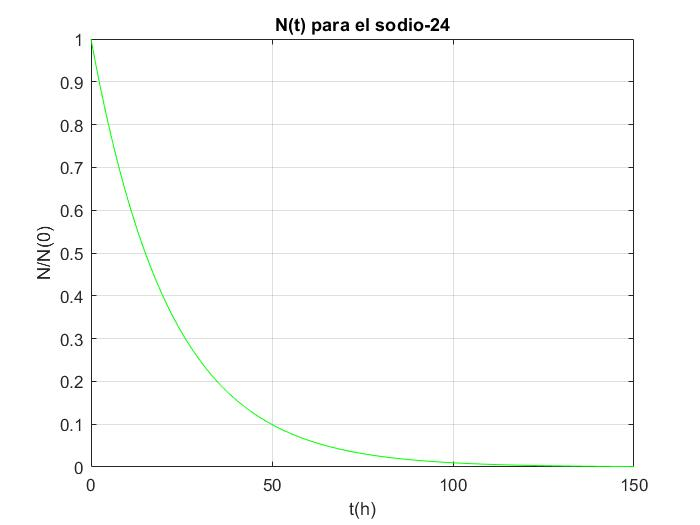
\includegraphics[scale=0.5]{imagenes/decaimiento_sodio_24.jpg}
        \caption{Gráfica del decaimiento exponencial del sodio-24 en en un intervalo de 150 horas.}
        \label{decaimientodelsodio24}
    \end{center}
\end{figure*}

\subsection{Desintegración en cadena}


\subsection{Ecuaciones de Bateman}

\noindent Las ecuaciones de Bateman son un sistema de ecuaciones diferenciales ordinarias propuestas por el matemático británico Harry Bateman en 1910 para generalizar las cadenas de desintegración del tipo $Padre\rightarrow Hijo \rightarrow Nieto$ \cite{Podgorsak.2016}.

\noindent Debido a que la cantidad de núcleos que participan en el proceso de desintegración es tan grande, podemos suponer que la función $N=N(t)$ que da el número de núcleos en un tiempo $t$ es una función continua, no discreta. De esta manera, es posible aplicar sobre ella las reglas de cálculo como ya las conocemos \cite{Podgorsak.2016}. 

\noindent Siguiendo a \textit{Podgorsak} en \cite{Podgorsak.2016}, tenemos que la cadena de desintegración descrita en el modelo de Bateman comprende las siguientes condiciones iniciales:

\begin{equation}
    \eval{N_1(t)}_{t=0}=N_1(0)\neq 0,\label{condicioninicialpadre}
\end{equation}
\begin{equation}
    N_2(0)=N_3(0)=...=N_i(0)=0, \label{condicioninicialproductos}
\end{equation}

\noindent como conveniencia para futuras referencias llamaremos a la ecuación \ref{condicioninicialpadre} \textit{condición inicial del núcleo padre} y a \ref{condicioninicialproductos}, \textit{condición inicial de los productos}. 

El significado o la implicación de las ecuaciones \ref{condicioninicialpadre} y \ref{condicioninicialproductos} es que, en un tiempo inicial, $t=0$, únicamente disponemos de los núcleos de la muestra padre para desintegración nuclear, mientras que los productos de su fisión permanecen inexistentes. Es solo hasta que el padre ha decaído que comenzamos a ver valores de $N$ distintos de cero para los elementos resultantes de la fisión. 

El número de núcleos disponibles en un tiempo $t$ para el k-ésimo producto de fisión viene dado por:

\begin{equation}
        N_k(t)=N_1(0) e^{-\lambda_1 t}+C_2 e^{-\lambda_2 t}+...+C_k e^{-\lambda_k t} \label{iesimonucleo}
\end{equation}

\noindent Donde $N_1^{(0)}$ es el número inicial de núcleos de la muestra radiactiva. Para los valores numéricos de los coeficientes $C_k$ de Bateman, \textit{Flanagan y Senftle} en \cite{Flanagan1954} ofrecen tablas completas de los términos que involucran.

En general, \cite{Loch.2013} ofrece una generalización más compacta válida para cualquier núcleo en la secuencia:

\begin{equation}
        N_m(t)=N_1^{(0)} \prod_{k=1}^{m-1}\lambda_k\sum_{j=1}^{m}\left(\frac{e^{\lambda_j t}}{\prod\limits_{p=1, p\neq j}^{m}\left(\lambda_p-\lambda_j\right)}\right) \label{batemangeneral}
\end{equation}

De acuerdo con \textit{Pratiwi et al} en \cite{Pratiwi.2021}, Bateman habría resuelto sus ecuaciones con transformadas de Laplace, y este método sería efectivo para sistemas lineales \textit{bien portados}, pero en el caso de reacciones en cadena con bifurcaciones en los productos de desintegración sumado a constantes de desintegración diferentes para cada producto, el sistema requiere de un tratamiento matricial numérico. 